\section{Dimension Reduction}
\label{sec:dimred}

In the previous section we created a $43266 \times 468$ matrix containing binary values encoding the survey responses of all individuals. Let us denote this matrix \verb|mat|. In the rest of this analysis our goal is to extract information about how these individuals can be clustered into groups based on their dialects. It is often cumbersome and opaque to work in a space of $468$ dimensions and further it is unlikely that all $468$ variables are actually important in the questions we are trying to answer. To this end we shall in this section we investigate various dimension reduction techniques. Our goal is to reduce the ambient dimension from $468$ to a manageable number.

In investigating various methods of dimension reduction and comparing them against each other, we need to decide on how to compare clusterings. For instance let $c^1$ and $c_2$ denote two possible clusterings of $n$ data points (in this case, $n = 43266$ individuals). That is, $c^1_i$ is an integer denoting the cluster to which $i^{th}$ individual has been allocated in the first clustering. We could of course visualize both clusters in separate plots (how to do this is still a question since we are sitting in a large dimensional space), and then visually inspect how close they are. But this requires human intervention and is both time-consuming and subjective.

Instead, we use the notion of Rand index \cite{randindex} to compute the similarity of two clusterings. Rand index can be defined using the following expression,
$$
R(c^1,c^2) = \frac{a+b}{{n \choose 2}}
$$
where $a$ is the number of pairs of individuals who are clustered together in both $c^1$ and $c^2$ and $b$ is the number of pairs of individuals who are clustered separately in both $c^1$ and $c^2$. Note that the denominator is simply the total number of pairs of individuals. In the above definition the number of clusters in $c^1$ and $c^2$ need not be same. Mathematically, the Rand index can be written as below, where for a set $S$, its cardinality is denoted by $|S|$, and the $i^{th}$ individual is dentoed by $x_i$,
$$
R(c^1,c^2) = \frac{|\{(i,j)|c^1_i = c^1_j, c^2_i = c^2_j \}| + |\{(i,j)|c^1_i \neq c^1_j, c^2_i \neq c^2_j \}|    }{{n \choose 2}}
$$

It can be observed that $0 \leq R \leq 1$ always and $R = 1$ iff the two clusterings are equivalent.

In the following subsections, we begin computing various sketched versions of \verb|mat|. In order to judge the performance of such reductions, we can and will use some visual inspection. But, to get more quantified results, we will use the following scheme: let \verb|reducedmat| denote a sketch of \verb|mat| produced by a generic dimension reduction technique. We will compute k-means clusterings based on both the full data \verb|mat| and the reduced data \verb|reducedmat| and compare the similarity of these two clusterings via Rand index.

For this analysis, we will primarily fix $k=4$. This number is arrived at by gap statistic analysis and visual inspection of the result of k-means on full data. More details on this are forthcoming in later sections.

\subsection{Principal Component Analysis}

The first technique we shall investigate is PCA. To decide on the number of PC's, we gather all principal components and their variance from \verb|mat|. The variances and cumulative variances of the principal components are shown in Figure \ref{fig:pcvars}.

\begin{figure}[ht]
	\centering
	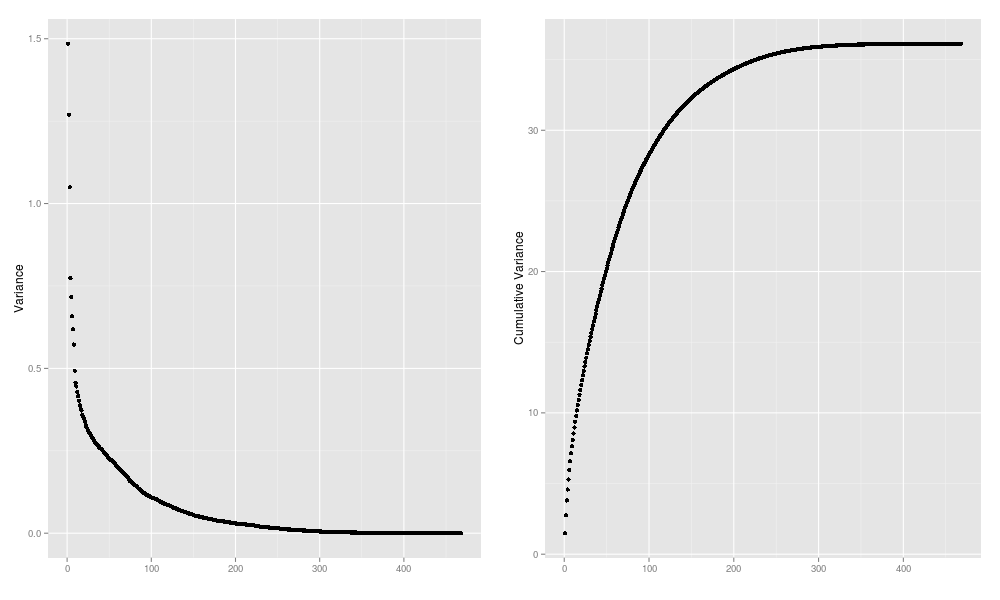
\includegraphics[width=0.8\textwidth]{fig/plot1.png}
	\caption{Variance and Cumulative Variance of Principal Components}
	\label{fig:pcvars}
\end{figure}


\begin{figure}[ht]
	\centering
	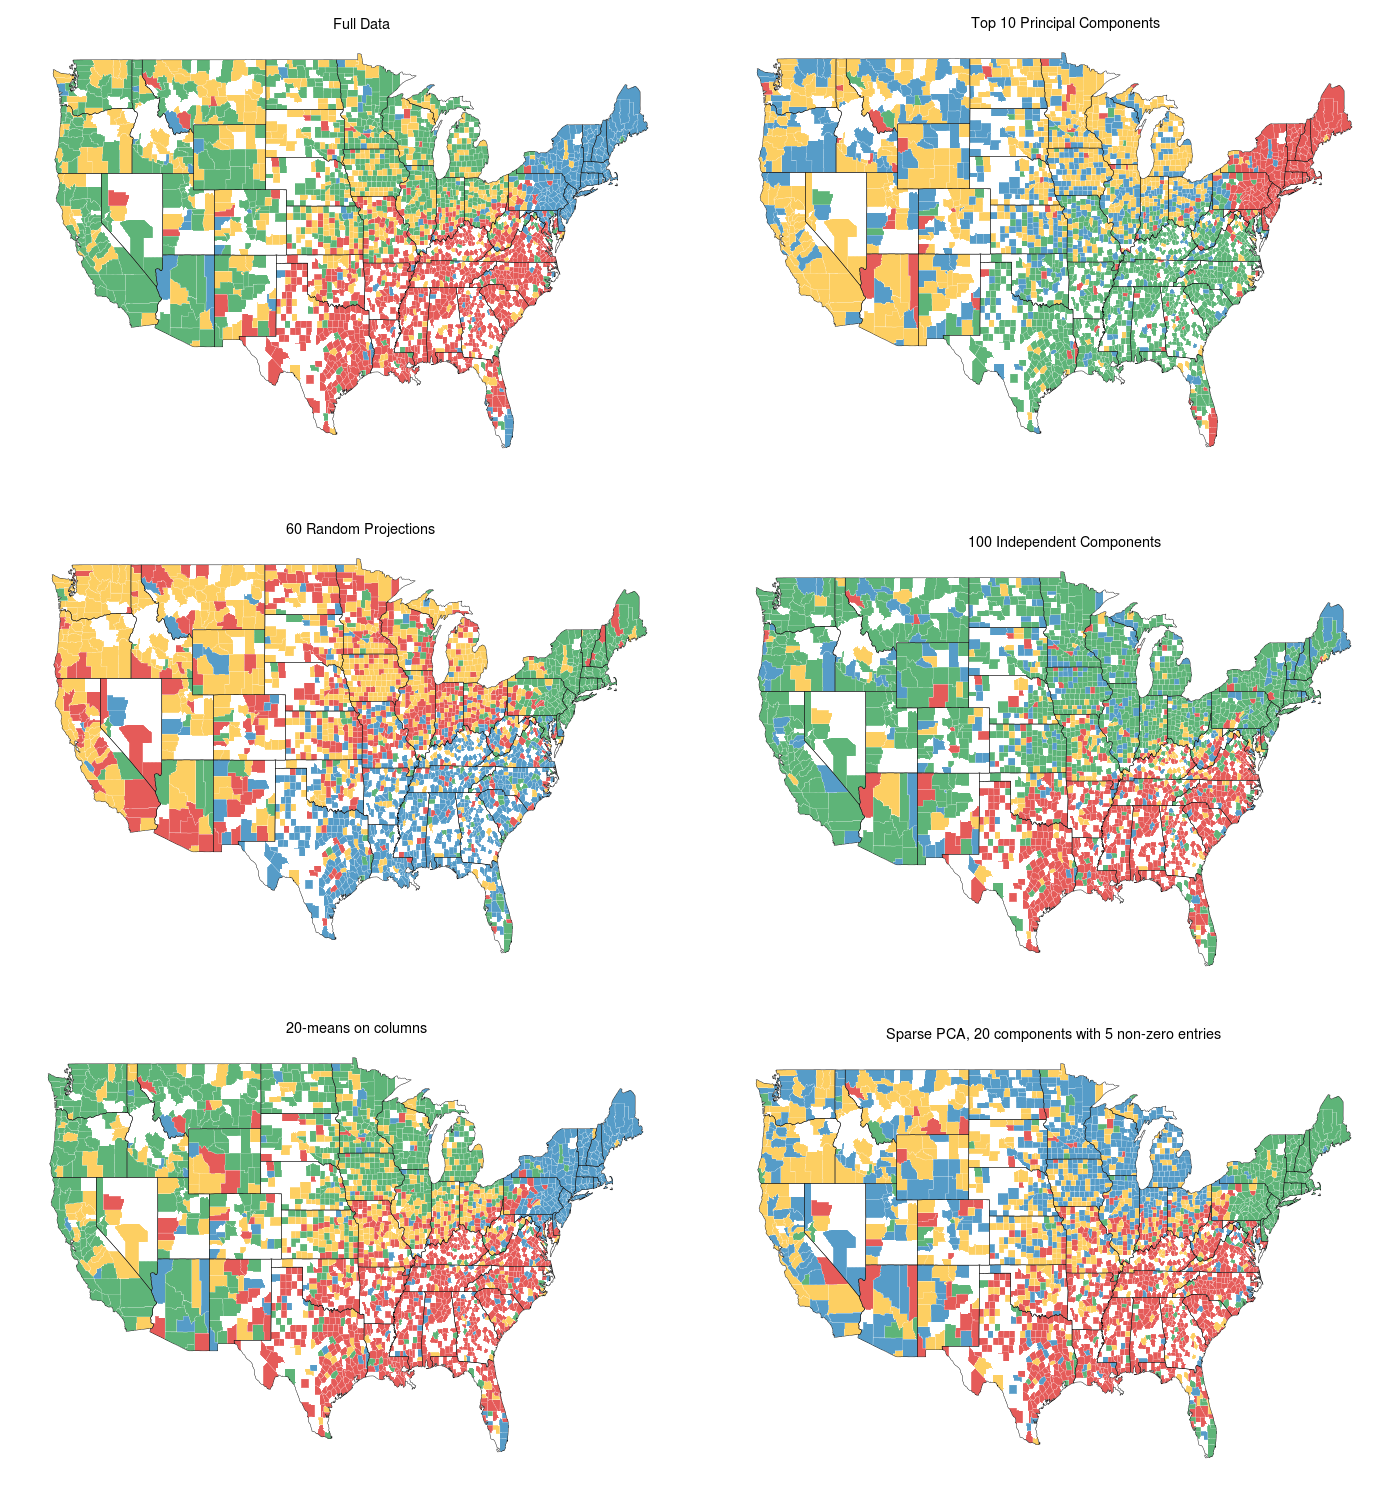
\includegraphics[width=0.8\textwidth]{fig/plot2to6.png}
	\caption{Comparison of 4-means clustering results on full data and various dimension reduction approaches. From top left in row major order: Full data, top $10$ principal components,}
	\label{fig:allplots}
\end{figure}

Observe that, the principal components do not show a sharp dropoff in variance, indicating that there is no small dimensional linear subspace which contains almost all of the variance in \verb|mat|. Dimension reduction by PCA is not likely to be very helpful in this data since we will need a lot of principal components in order to capture the full shape of the data.

Next we compute the k-means output of full data and top $10, 50, 100, 150, 200$ principal components. To save space for more interesting visualizations later in the document, we refrain from including the output visually at this point. We can compare the Rand index at each level of reduction. It is found that the Rand indices are \verb|0.96 0.99 0.84 0.80 0.80|. This makes using the top $10$ PC's quite desirable even though they explain only $20\%$ of the variance of the data. Note that the Rand indices are inherently random since the initial point of $k$-means algorithm is random. We shall revisit this consideration later. But this leads us to our next discussion. Fixing the number of principal components apriori does not tell us how much of the original variability in the data has been captured by the data. In the next sequence of plots, we investigate with top PC's chosen so that they explain $50\%, 80\%$ and $90\%$ of the data (the number of PC's required are $42, 106$ and $155$ respectively). In this case, the Rand indices come out as \verb|0.94 0.99 0.93|, further indicating that
\begin{center}
\verb|mat| possibly retains a fair amount of noise and using principal components can clean the data
\end{center}

This is corroborated by the fact that smaller number of PC's actually lead to a better Rand index even though they capture only a small proportion of the total variance. Figure \ref{fig:allplots} shows visual outputs of using full data and top $10$ principal components. In the generation of these plots, after getting cluster assignments for individual persons using $4$-means on either the full data or the top $10$ PC's, we further process to generate cluster assignments for all the counties present in the dataset and plot these on a map of United States.
\begin{center}
To get cluster assignments for each county given the cluster assignments of all individuals, we look at the list of all individuals residing in a particular county and take majority vote of their cluster assignments
\end{center}


\subsection{Random Projections}

Random projections are an widely used, versatile and efficient dimension reduction specially suited for unsupervised learning problems such as this. Using random projections, one can project rows of \verb|mat| into a randomly constructed subspace of dimension $m$ by taking linear combinations. The celebrated Johnson-Lindenstrauss lemma guarantees that with probability at least $1-\delta$, all norms and inner products after projections are preserved within an accuracy of $\epsilon$ of their original values as long as the number of projections $m$ is $\mathcal{O}(\log(n/\delta)/\epsilon^2)$. Since $k$-means and many other unsupervised learning methods operate only on the distances between data points, it is believable that the clusterings computed from the projected data would be closely related to the clusterings computed from full data. We now investigate this theoretical intuition using $20,40,60,120$ projections. It is worthwhile to note that \verb|log(43266)=10.67|. The Rand indices of these sequences of dimension reductions are \verb|0.64 0.69 0.76 0.78|. Figure \ref{fig:allplots} shows a visual comparison of the outputs of k-means of full data and on $120$ random projections.

\begin{center}
This would seem to further corroborate the notion that not all columns of \verb|mat| are equally important in constructing geographically meaningful clusters. Using a few top principal components succeeds in encapsulating the important components better than random projections which aims to preserve every component with equal importance. We will return to this issue in later sections when we discuss which survey questions are more dominant in constructing a geographical divide than others
\end{center}

\subsection{Independent Component Analysis}

A different approach to dimension reduction is using Independent Component Analysis, which aims to describe as a few components which contain a lot of the signal and consequently have a non-gaussian distribution and a lot of other directions which are mostly noisy and consequently more gaussian. ICA iteratively chooses directions with maximal non-gaussianity and projects the data along those directions. Here we try our now established method on $10, 30, 50, 100$ top independent components. The resulting Rand indices are \verb| 0.59 0.56 0.56 0.66|. Figure \ref{fig:allplots} shows the maps comparing k-means on full data with k-means on top 100 IC's
The results are quite lacklustre and do not add much to our present understanding of the data. It is perhaps justified to conclude that the interesting directions of this data are gaussian in nature.

\subsection{$k$-means as a dimension reduction technique}

An interesting idea is posed in this subsection. The columns of \verb|mat| are constructed by binarising responses to a survey. As such similar questions would lead to similar columns in \verb|mat| and it is believable that all $468$ columns of \verb|mat| do not really need to be treated separately. In fact, based on our analysis till now it is quite likely that being able to remove some noise from the columns of \verb|mat| would clean the results of clustering. One way to achieve all this to cluster the columns of \verb|mat| (in contrast to the rows, which is the problem we have been concentrating). This clustering can be performed using k-means as an illustration. After clustering, each column is replaced by its cluster mean and usual k-means can be performed on this modified matrix. This is equivalent to performing k-means with a weighted distance function on the matrix of the column cluster centers. The weights in the distance function come from the sizes of the column clusters. To be precise, if $Y$ is the new \verb|reducedmat| computed using this method, then columns of $Y$ are the cluster centers and denoting by $n_j$ the number of columns mapped to the $j^{th}$ cluster (whose center is the $j^{th}$ column of $Y$), two rows $y_i$ and $y_{i'}$ would have the following distance associated with them,
$$
d(y_i,y_{i'}) = \sqrt{\sum_j n_j (y_{ij}-y_{i'j})^2}
$$
An important point to note in this regard is since the standard k-means algorithm deals in squared distances $d^2(.,.)$ where $d$ is defined above, it is important to pass $\sqrt{n_j}$ as weights to the algorithm. The results when the columns are clustered into $5,10,20$ clusters are computed. The Rand indices are \verb|0.70 0.74 0.77|. Figure \ref{fig:allplots} compares the outputs of k-means on full data with k-means on columns clustered with $20$-means. The results look quite satisfactory.

\subsection{Sparse PCA}

Insert few words on sparse PCA. Figure \ref{fig:allplots}

\subsection{Overview of dimension reduction techniques}

In this preliminary investigation, we conclude that performing dimension reduction via either PCA or $k$-means on the columns of \verb|mat| would produce satisfactory results in this problem. The reasoning behind this conclusion is likely the excess noise carried by the $468$ columns of \verb|mat|. The next section provides insight into our tinkerings with different clustering methods in conjunction with different dimension reductions to gain further insight into the data before we make taller claims.
